\documentclass[tikz,dvisvgm]{standalone}

\usetikzlibrary{positioning}

\begin{document}

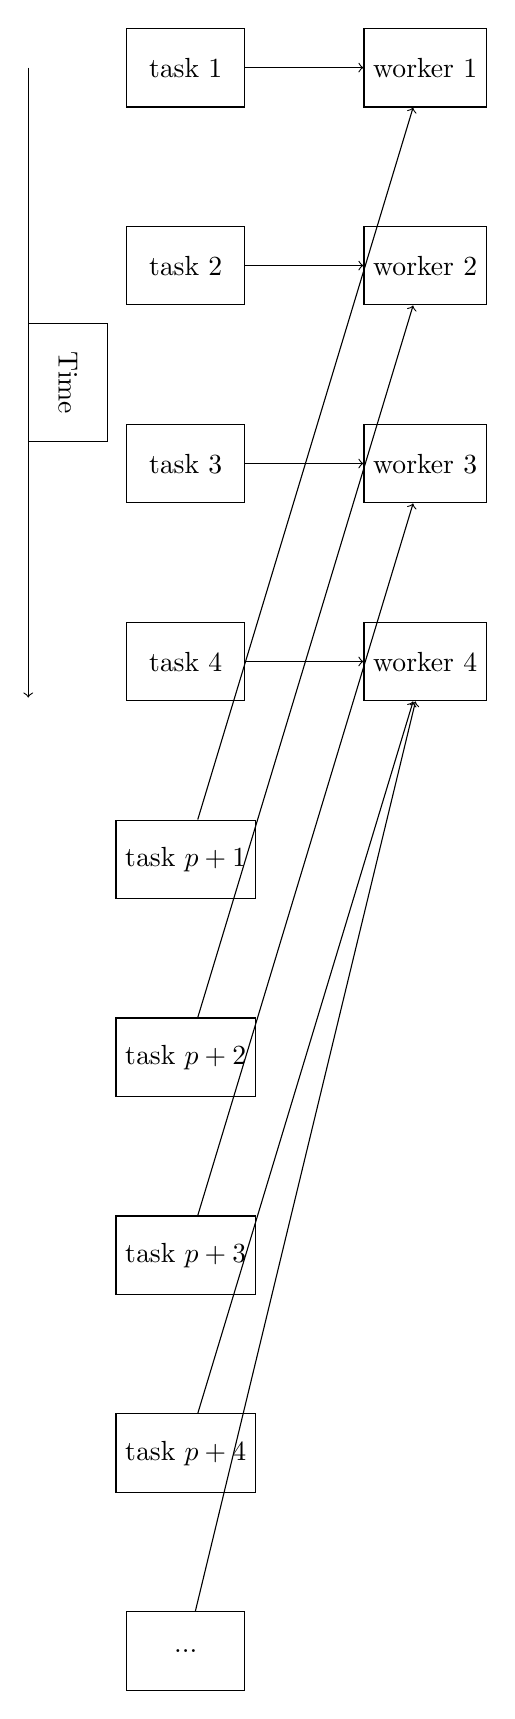
\begin{tikzpicture}[node distance=1.5cm, every node/.style={draw, minimum width=1.5cm, minimum height=1cm}]
  \node (t1) at (0,0) {task 1};
  \node (t2) [below=of t1] {task 2};
  \node (t3) [below=of t2] {task 3};
  \node (t4) [below=of t3] {task 4};
  \node (tp1) [below=of t4] {task $p+1$};
  \node (tp2) [below=of tp1] {task $p+2$};
  \node (tp3) [below=of tp2] {task $p+3$};
  \node (tp4) [below=of tp3] {task $p+4$};
  \node (dots) [below=of tp4] {...};
  \node (w1) [right=of t1] {worker 1};
  \node (w2) [right=of t2] {worker 2};
  \node (w3) [right=of t3] {worker 3};
  \node (w4) [right=of t4] {worker 4};
  \draw [->] (t1) -- (w1);
  \draw [->] (t2) -- (w2);
  \draw [->] (t3) -- (w3);
  \draw [->] (t4) -- (w4);
  \draw [->] (tp1) -- (w1);
  \draw [->] (tp2) -- (w2);
  \draw [->] (tp3) -- (w3);
  \draw [->] (tp4) -- (w4);
  \draw [->] (dots) -- (w4);
  \draw [->] (-2,0) -- (-2,-8) node [midway, above, sloped] {Time};
\end{tikzpicture}

\end{document}